\documentclass[11pt]{article}

\usepackage[margin=1in]{geometry}
\usepackage{amsmath}
\usepackage{amssymb}
\usepackage{amsthm}
\usepackage{mathtools}
\usepackage{graphicx}
\usepackage[utf8]{inputenc}
\usepackage[T1]{fontenc}
\usepackage{lmodern}
\usepackage{microtype}
\usepackage[hidelinks]{hyperref}

% Theorem environments
\newtheorem{proposition}{Proposition}
\newtheorem{theorem}{Theorem}
\newtheorem{corollary}{Corollary}
\newtheorem*{remark}{Remark}

% Operator names
\DeclareMathOperator{\Tr}{Tr}
\DeclareMathOperator{\diag}{diag}
\DeclareMathOperator{\Var}{Var}
\DeclareMathOperator{\Cov}{Cov}

% Convenient commands
\newcommand{\R}{\mathbb{R}}
\newcommand{\bkt}{\mathrm{bkt}}
\newcommand{\rel}{\mathrm{rel}}
\newcommand{\ind}{\mathrm{ind}}
\newcommand{\cm}{\mathrm{cm}}
\newcommand{\nc}{\mathrm{nc}}
\newcommand{\sep}{\mathrm{sep}}
\newcommand{\one}{\mathbf{1}}
\newcommand{\transp}{^{\!\top}}

\title{Loss-Versus-Rebalancing Reduced in\\Cross-Correlated Multi-Asset LMSR Pools}
\author{Tim Olson\thanks{\texttt{timolsoncrypto@gmail.com}} \and Claude Opus 4.7}
\date{}

\begin{document}
\maketitle

\begin{abstract}
We derive in closed form the instantaneous loss-versus-rebalancing (LVR) rate for the multi-asset Hanson LMSR with $N$ risky assets, one num\'eraire, and an arbitrary positive semi-definite return-covariance matrix $\Sigma$, under the standard idealized assumption of frictionless continuous arbitrage. The rate decomposes as the sum of the LVR rates of $N$ independent two-asset LMSR pools minus a non-negative \emph{cross-correlation discount} of closed form $\tfrac{b}{2(1+S)}\,P\transp\Sigma P$, where $S$ is the total risky value held by the pool. Equivalently, the rate splits orthogonally into an idiosyncratic relative-mode variance term plus a single basket-vs-num\'eraire common-mode term, making the simplex's role as a covariance projector for coherent basket motion explicit. For perfectly correlated equal-volatility assets the discount cancels the entire relative-mode contribution: an $(N{+}1)$-asset balanced pool has the same LVR rate as a two-asset LMSR with matched liquidity parameter $b$ and matched risky notional $S$, and a no-num\'eraire pool of perfectly correlated assets has zero LVR. The discount has no analog in \emph{separable} bilateral CFMMs of any local curvature: it descends from the off-diagonal simplex-coupling term in $\nabla^2 V$ induced by the shared constraint $\sum p_i = 1$, and off-diagonal Hessian structure is necessary (though we do not establish it sufficient) for any discount of this form.
\end{abstract}

\section{Introduction}

Milionis, Moallemi, Roughgarden, and Zhang (2024) introduced the \emph{loss-versus-rebalancing} (LVR) metric to quantify the rate at which a constant-function market maker (CFMM) bleeds value to arbitrageurs in the presence of a frictionless external reference market. Their value-function methodology applies to any CFMM whose pool value $V(P)$ is a $C^2$ concave function of the external price vector $P$: under idealized continuous arbitrage and an It\^o price process with log-return covariance matrix $\Sigma$, the instantaneous LVR rate is
\begin{equation*}
\ell(P) \;=\; -\tfrac{1}{2}\sum_{i,j} P_i P_j \,\Sigma_{ij}\, \frac{\partial^2 V}{\partial P_i\,\partial P_j}. \tag{0}
\end{equation*}
For the canonical two-asset constant-product AMM with single-asset log-return volatility $\sigma$, the rate evaluates to $\ell = (\sigma^2/8)\,V$.

Throughout this paper we adopt the same idealization: continuous, frictionless, infinitesimal arbitrage at every instant. Real systems incur latency, gas, discrete trade sizes, and finite arbitrage cadence; the rate $\ell(P)$ should accordingly be read as an \emph{instantaneous, infinitesimal-arbitrage benchmark} rather than a quantity directly observable in deployed pools. The benchmark is nevertheless useful because it cleanly isolates the effect of pool geometry on adverse selection by arbitrageurs; fee and discretization corrections enter multiplicatively as in Milionis et al.\ (2024) and preserve the geometric structure derived here.

The Logarithmic Market Scoring Rule (LMSR) of Hanson (2003, 2007) is the canonical \emph{multi-asset} automated market maker, originally designed for prediction markets where $N+1$ outcomes share a single simplex of marginal probabilities. Deployed as a generic AMM with one num\'eraire and $N$ risky assets, the LMSR maintains $N(N+1)/2$ simultaneously-quoted pairwise exchange rates, all derived from a single shared state vector $q \in \R^{N+1}$. A trade against one pair necessarily moves every other pair's marginal price as well, propagating price information across the entire simplex. This is the geometric coupling absent in any system of disjoint bilateral pools.

We show that this propagation has a quantitatively precise consequence for LVR. Our main result, eq.~$(\dagger)$ in \S\ref{sec:lvr}, is
\[
\ell(P) \;=\; \underbrace{\frac{b}{2}\sum_{i=1}^N \sigma_i^2 P_i}_{\text{sum of $N$ two-asset LMSR rates}} \;-\; \underbrace{\frac{b}{2(1+S)}\,P\transp\Sigma P}_{\text{cross-correlation discount}}, \qquad S \equiv \sum_{i=1}^N P_i.
\]
The discount is non-negative for any PSD $\Sigma$ and grows with the variance of the value-weighted basket return. In \S\ref{sec:lvr} we show that this rewrites as a clean common-mode/relative-mode split (Theorem~\ref{thm:cm}): the LVR rate equals a relative-mode piece $\tfrac{b}{2}\sum_i P_i\,\Var(r_i - \bar r)$ plus a single common-mode piece $\tfrac{bS}{2(1+S)}\,\Var(\bar r)$, where $\bar r$ is the value-weighted basket return. For perfectly correlated equal-volatility assets, the relative-mode piece vanishes and only the common-mode-versus-num\'eraire term remains, collapsing the multi-asset LVR to that of a single synthetic two-asset pool. In a pool with no num\'eraire, both the common-mode arbitrage channel and the relative-mode contribution can vanish simultaneously, and perfect correlation drives LVR to exactly zero.

The cross-correlation discount is structural in a precise sense: it descends from the off-diagonal simplex-coupling term in $V$'s Hessian (eq.~(6) in \S\ref{sec:hessian}) induced by the constraint $\sum p_i = 1$. By Proposition~\ref{prop:sep}, any \emph{separable} bilateral CFMM --- one whose pool value decomposes as $V(P) = \sum_i V_i(P_i)$ --- has a diagonal Hessian and therefore cannot exhibit a covariance-canceling term of this form. Equivalently, off-diagonal Hessian structure is \emph{necessary} for a discount of this form. We do not claim, and our analysis does not establish, that non-LMSR multi-asset CFMM constructions (entropic, CES-like, weighted-softmax, or otherwise) cannot exhibit analogous off-diagonal couplings or that the LMSR is unique in admitting such a discount; characterizing the full class of multi-asset CFMMs that do is a separate question we do not undertake here.

Beyond its immediate AMM-theoretic content, the result fits naturally within the convex-analytic / Bregman-geometric view of scoring-rule market makers (Abernethy, Chen, \& Vaughan 2013; Frongillo \& Reid 2015), of which LMSR is the canonical instance.

The remainder of the paper is organized as follows. \S\ref{sec:setup} fixes notation in Hanson's shares-outstanding convention used by Milionis et al. \S\ref{sec:value} derives the closed-form pool value function $V(P)$ at continuous-arbitrage equilibrium. \S\ref{sec:hessian} computes its Hessian. \S\ref{sec:lvr} substitutes into the master LVR formula~(0), exhibits the decomposition~$(\dagger)$, the common-mode/relative-mode form (Theorem~\ref{thm:cm}), and the separable-CFMM comparison (Proposition~\ref{prop:sep}). \S\ref{sec:special} specializes to symmetric cases including the no-num\'eraire pool. \S\ref{sec:conclusion} concludes.

\section{Setup}\label{sec:setup}

We work in continuous time with $N+1$ assets: a num\'eraire (asset~$0$) with constant price $P_0 \equiv 1$, and $N$ risky assets with strictly positive prices $P = (P_1, \dots, P_N) \in \R^N_{>0}$ following correlated geometric Brownian motion,
\[
d\log P_i \;=\; \mu_i \, dt \;+\; \sum_{k=1}^N \Sigma^{1/2}_{ik}\, dW^{(k)}_t, \qquad \langle d\log P_i,\, d\log P_j \rangle \;=\; \Sigma_{ij}\, dt,
\]
with $\Sigma \in \R^{N\times N}$ symmetric positive semi-definite. We write $\Sigma_{ij} = \rho_{ij}\sigma_i \sigma_j$, so $\Sigma_{ii} = \sigma_i^2$. Throughout, $r_i \equiv d\log P_i$ denotes the instantaneous log return of asset~$i$.

\paragraph{Cost function.} The Hanson LMSR cost function on state $q = (q_0, q_1, \dots, q_N) \in \R^{N+1}$ is
\[
C(q) \;=\; b \log \sum_{i=0}^N \exp(q_i/b), \qquad b > 0.
\]
Following Hanson's shares-outstanding convention (as adopted by Milionis et al.), $q_i$ is the cumulative quantity of asset~$i$ the market maker has sold to traders; the MM is short $q_i$ of asset~$i$. The marginal simplex price of asset~$i$ is
\[
p_i(q) \;=\; \frac{\partial C}{\partial q_i} \;=\; \frac{e^{q_i/b}}{\sum_k e^{q_k/b}}, \qquad \sum_{i=0}^N p_i \;=\; 1.
\]
Trading from state $q$ to $q + dq$ collects cash $dC = \sum_i p_i\, dq_i$. Over a finite history from initial state $q^{(0)}$, the MM holds cash $C(q) - C(q^{(0)})$ and is short $q_i$ of each asset.

\paragraph{Net pool value.} At external prices $P = (1, P_1, \dots, P_N)$, the MM's mark-to-market is
\begin{equation*}
V(q; P) \;=\; \bigl[C(q) - C(q^{(0)})\bigr] \;-\; \sum_{i=0}^N q_i P_i. \tag{1}
\end{equation*}
The constant $-C(q^{(0)})$ does not depend on $P$ and drops from $\nabla^2 V$ and from the LVR rate; we omit it throughout.

\paragraph{Continuous arbitrage equilibrium.} We assume frictionless continuous arbitrage: at every instant the pool's marginal prices match the external prices, so $p_i(q)/p_0(q) = P_i/1$. Combined with $\sum_i p_i = 1$,
\begin{equation*}
p_0(q^\star) \;=\; \frac{1}{1+S}, \qquad p_i(q^\star) \;=\; \frac{P_i}{1+S} \quad (i \ge 1), \qquad S \equiv \sum_{i=1}^N P_i. \tag{2}
\end{equation*}

\paragraph{Coordinate redundancy.} The simplex prices $p_i(q)$ are invariant under the shift $q \to q + c\one$ (softmax translation invariance), so $q^\star$ is determined only up to an additive constant. We fix it by imposing $C(q^\star) = C_0$, giving $q_i^\star = C_0 + b\log p_i$ and, substituting~(2),
\begin{equation*}
q_0^\star(P) \;=\; C_0 - b\log(1+S), \qquad q_i^\star(P) \;=\; C_0 + b\log\!\frac{P_i}{1+S} \quad (i \ge 1). \tag{3}
\end{equation*}
Using $C(q + c\one) = c + C(q)$, a one-line check shows that the choice of $C_0$ shifts $V$ by the $P$-linear amount $-C_0 S$ and is therefore immaterial for $\nabla^2_P V$ and the LVR rate~(0). We drop linear-in-$P$ remainders throughout.

\section{Arbitrage Equilibrium and Pool Value Function}\label{sec:value}

Substituting~(3) into~(1) and using $C(q^\star) = C_0$:
\[
V(P) \;=\; C_0 \;-\; \sum_{i=0}^N q_i^\star(P) P_i.
\]
Expand:
\begin{align*}
\sum_{i=0}^N q_i^\star P_i
&\;=\; q_0^\star \;+\; \sum_{i=1}^N q_i^\star P_i \\
&\;=\; \bigl[C_0 - b\log(1+S)\bigr] \;+\; \sum_{i=1}^N\bigl[C_0 + b\log P_i - b\log(1+S)\bigr] P_i \\
&\;=\; C_0(1+S) \;-\; b(1+S)\log(1+S) \;+\; b\sum_{i=1}^N P_i \log P_i.
\end{align*}
Therefore
\[
V(P) \;=\; -C_0 S \;+\; b(1+S)\log(1+S) \;-\; b\sum_{i=1}^N P_i \log P_i.
\]
The first term, $-C_0 S$, is linear in $P$ and drops from $\nabla^2 V$. We retain only the relevant part:
\begin{equation*}
\boxed{\;\; V(P) \;=\; b\,(1+S)\log(1+S) \;-\; b\sum_{i=1}^N P_i \log P_i \pmod{\text{linear in }P}. \;\;} \tag{4}
\end{equation*}

\begin{remark}
Equation~(4) reduces to the standard two-asset Hanson value function $V(P) = b(1+P)\log(1+P) - bP\log P$ when $N = 1$.
\end{remark}

\begin{remark}
Equation~(4) sits inside the broader convex-analytic / Bregman-geometric view of scoring-rule market makers (Abernethy, Chen, \& Vaughan 2013; Frongillo \& Reid 2015); concavity of $V$ in external prices is dual to strict convexity of the LMSR log-partition function in its natural state parameters. We do not develop the duality further here.
\end{remark}

\section{The Hessian}\label{sec:hessian}

Differentiating~(4):
\begin{equation*}
\frac{\partial V}{\partial P_i} \;=\; b\log(1+S) + b - b\log P_i - b \;=\; b\log\!\frac{1+S}{P_i} \pmod{\text{const}}. \tag{5}
\end{equation*}
Differentiating again:
\[
\frac{\partial^2 V}{\partial P_i\,\partial P_j} \;=\; \frac{b}{1+S} \;-\; \frac{b}{P_i}\,\delta_{ij},
\]
or, in matrix form with $\one = (1, \dots, 1)\transp$,
\begin{equation*}
\boxed{\;\; H(P) \;\equiv\; \nabla^2 V(P) \;=\; \frac{b}{1+S}\,\one\one\transp \;-\; b\,\diag(P_i^{-1}). \;\;} \tag{6}
\end{equation*}

\begin{proposition}[Strict concavity]\label{prop:concave}
$V$ is strictly concave on $\R^N_{>0}$.
\end{proposition}
\begin{proof}
By Cauchy--Schwarz, $\bigl(\sum_i x_i\bigr)^2 = \bigl(\sum_i (x_i/\sqrt{P_i})\sqrt{P_i}\bigr)^2 \le S\sum_i x_i^2/P_i$. Hence
\[
x\transp(-H)\,x \;=\; b\sum_i \frac{x_i^2}{P_i} - \frac{b}{1+S}\Bigl(\sum_i x_i\Bigr)^{\!2} \;\ge\; \frac{b}{1+S}\sum_i \frac{x_i^2}{P_i} \;>\; 0
\]
for $x \ne 0$.
\end{proof}

\paragraph{Structural observation.} Equation~(6) decomposes $H$ into a rank-one coupling $\tfrac{b}{1+S}\one\one\transp$ minus a diagonal piece $-b\,\diag(P_i^{-1})$. The diagonal piece is the same local curvature that would be obtained from $N$ isolated two-asset LMSRs at the same liquidity~$b$. The off-diagonal piece --- uniform entries $H_{ij} = b/(1+S)$ for every $i \ne j$ --- is the \emph{shared-simplex channel}: an arbitrage against asset~$i$ adjusts the simplex weight $p_0$ of the num\'eraire and thereby moves the marginal exchange rate of every other asset~$j$. As we will see, this coupling is exactly what produces the cross-correlation discount in~$(\dagger)$.

\section{LVR Master Formula}\label{sec:lvr}

We now substitute~(6) into the value-function LVR formula and develop three equivalent forms of the resulting expression: the independent-pair / discount decomposition~$(\dagger)$, the common-mode / relative-mode form (Theorem~\ref{thm:cm}), and a trace form $\ell(P) = \tfrac{b}{2}\Tr[M(P)\,\Sigma]$ that makes the geometric content transparent. We close the section with the separable-CFMM comparison (Proposition~\ref{prop:sep}).

\subsection{The master decomposition}

By Milionis et al.\ (2024, Theorem~1), specialized to~(0), the instantaneous LVR rate of a CFMM with $C^2$ concave value function $V(P)$ under an It\^o price process with $\langle dP_i, dP_j\rangle = P_i P_j \Sigma_{ij}\,dt$ is
\begin{equation*}
\ell(P) \;=\; -\tfrac{1}{2}\sum_{i,j=1}^N P_i P_j \,\Sigma_{ij}\, H_{ij}(P). \tag{7}
\end{equation*}
Our equilibrium $V(P)$ in~(4) is $C^\infty$ on $\R^N_{>0}$ and strictly concave (Proposition~\ref{prop:concave}), so the regularity hypotheses of Milionis et al.'s Theorem~1 are satisfied. The right-hand side is non-negative because $-H$ is PSD and $\Sigma$ is PSD. Substituting~(6):
\begin{align*}
\ell(P)
&\;=\; -\tfrac{1}{2}\sum_{i,j} P_i P_j \Sigma_{ij}\Bigl[\frac{b}{1+S} - \frac{b}{P_i}\,\delta_{ij}\Bigr] \\
&\;=\; \frac{b}{2}\sum_i \Sigma_{ii}\, P_i \;-\; \frac{b}{2(1+S)}\sum_{i,j} P_i P_j \Sigma_{ij},
\end{align*}
which we package as
\begin{equation*}
\boxed{\;\; \ell(P) \;=\; \underbrace{\frac{b}{2}\sum_{i=1}^N \sigma_i^2 P_i}_{\ell_{\ind}(P)} \;-\; \underbrace{\frac{b}{2(1+S)}\, P\transp\Sigma P}_{\Delta(P)}. \;\;} \tag{$\dagger$}
\end{equation*}

\paragraph{Independent-pair benchmark $\ell_{\ind}(P)$.} This is the value of~(7) when $H$ is replaced by its diagonal $-b\,\diag(P_i^{-1})$ --- equivalently, the LVR rate of $N$ isolated (num\'eraire, asset~$i$) two-asset LMSRs at liquidity~$b$, summed across~$i$.

\paragraph{Cross-correlation discount $\Delta(P)$.} The amount removed by the simplex-coupling term in $H$. Because $\Sigma$ is PSD, $P\transp\Sigma P \ge 0$ for every covariance structure, so
\[
\Delta(P) \;\ge\; 0 \qquad\text{and}\qquad \ell(P) \;\le\; \ell_{\ind}(P) \quad \text{unconditionally}.
\]

\subsection{Basket-variance and trace forms}

Let $w_i = P_i/S$ be the value-weighted risky-asset weights and $\bar r = w\transp r$ the basket return, with variance
\[
\sigma_{\bkt}^2 \;\equiv\; \Var(\bar r) \;=\; w\transp\Sigma w.
\]
Then $P\transp\Sigma P = S^2\sigma_{\bkt}^2$ and $(\dagger)$ rewrites as
\begin{equation*}
\ell(P) \;=\; \frac{b}{2}\sum_i \sigma_i^2 P_i \;-\; \frac{b\, S^2}{2(1+S)}\,\sigma_{\bkt}^2. \tag{$\dagger'$}
\end{equation*}
In matrix language, with $D_P \equiv \diag(P)$,
\begin{equation*}
\ell(P) \;=\; \frac{b}{2}\Tr(D_P \Sigma) \;-\; \frac{b}{2(1+S)}\Tr(PP\transp\Sigma) \;=\; \frac{b}{2}\Tr\!\bigl[M(P)\,\Sigma\bigr], \tag{$\dagger''$}
\end{equation*}
where
\[
M(P) \;\equiv\; D_P \;-\; \frac{PP\transp}{1+S}
\]
is the LMSR's \emph{LVR operator}. It is PSD on $\R^N$: applying Cauchy--Schwarz with $u_i = x_i\sqrt{P_i}$ and $v_i = \sqrt{P_i}$,
\[
(P\transp x)^2 \;=\; \Bigl(\sum_i P_i x_i\Bigr)^{\!2} \;\le\; \Bigl(\sum_i P_i x_i^2\Bigr)\Bigl(\sum_i P_i\Bigr) \;=\; S\, x\transp D_P x,
\]
so $x\transp M(P)x = x\transp D_P x - (P\transp x)^2/(1+S) \ge \tfrac{1}{1+S}\,x\transp D_P x \ge 0$. Geometrically, $M(P)$ deflates the rank-one component of $\Sigma$ aligned with the price vector $P$, and the LVR rate is the trace inner product of this deflated covariance with the simplex-coupling structure.

\subsection{Common-mode / relative-mode decomposition}

The trace form~$(\dagger'')$ makes manifest that $\ell$ depends on $\Sigma$ only through the basket-direction projection and its complement. The following theorem packages this as a clean orthogonal split.

\begin{theorem}[Common-mode suppression]\label{thm:cm}
For each $i$, let $\sigma_{i,\rel}^2 \equiv \Var(r_i - \bar r)$ denote the variance of asset~$i$'s return relative to the value-weighted basket return $\bar r = w\transp r$, where $w_i = P_i/S$. Then $(\dagger)$ is equivalent to
\begin{equation*}
\boxed{\;\; \ell(P) \;=\; \underbrace{\frac{b}{2}\sum_{i=1}^N P_i\,\sigma_{i,\rel}^2}_{\ell_{\rel}(P)\ \text{--- relative-mode}} \;+\; \underbrace{\frac{b\, S}{2(1+S)}\,\sigma_{\bkt}^2}_{\ell_{\cm}(P)\ \text{--- common-mode}}. \;\;} \tag{$\ddagger$}
\end{equation*}
\end{theorem}
\begin{proof}
Direct algebra. Expand $\sigma_{i,\rel}^2 = \Var(r_i) - 2\,\Cov(r_i, \bar r) + \Var(\bar r) = \Sigma_{ii} - 2(\Sigma w)_i + \sigma_{\bkt}^2$. Multiply by $P_i$ and sum:
\[
\sum_i P_i\,\sigma_{i,\rel}^2 \;=\; \sum_i P_i \Sigma_{ii} \;-\; 2\sum_i P_i (\Sigma w)_i \;+\; S\,\sigma_{\bkt}^2.
\]
Using $\sum_i P_i (\Sigma w)_i = S\sum_i w_i(\Sigma w)_i = S\,w\transp\Sigma w = S\,\sigma_{\bkt}^2$,
\begin{equation*}
\sum_i P_i\,\sigma_{i,\rel}^2 \;=\; \sum_i P_i \Sigma_{ii} \;-\; S\,\sigma_{\bkt}^2. \tag{$\star$}
\end{equation*}
Therefore
\[
\frac{b}{2}\sum_i P_i \sigma_{i,\rel}^2 \;+\; \frac{b\,S}{2(1+S)}\sigma_{\bkt}^2
\;=\; \frac{b}{2}\sum_i \sigma_i^2 P_i \;-\; \frac{b\,S}{2}\sigma_{\bkt}^2 \;+\; \frac{b\,S}{2(1+S)}\sigma_{\bkt}^2,
\]
and combining the last two terms gives $-\tfrac{b\,S^2}{2(1+S)}\sigma_{\bkt}^2$, which is precisely $-\Delta(P)$ by~$(\dagger')$.
\end{proof}

The decomposition~$(\ddagger)$ is the precise mathematical content of the heuristic that LMSR's shared simplex ``filters out coherent basket motion'': the entire basket-variance contribution is captured by the single common-mode term $\ell_{\cm}$, which is the LVR rate one would compute for a two-asset LMSR holding the basket aggregate against the num\'eraire; the residual relative-mode term $\ell_{\rel}$ is driven only by idiosyncratic variances $\Var(r_i - \bar r)$ and is exactly the LVR that survives in the no-num\'eraire limit (\S\ref{sec:nocash}).

In factor-model language, $\bar r$ is a single systematic factor (the value-weighted basket return) and the residuals $r_i - \bar r$ are idiosyncratic deviations. $\ell_{\cm}$ is the systematic factor's LVR contribution charged exactly once --- as if the basket were a single synthetic asset --- and $\ell_{\rel}$ aggregates the idiosyncratic contributions weighted by the holdings~$P_i$.

\subsection{Separable bilateral CFMMs}

The discount in~$(\dagger)$ traces to the off-diagonal coupling in~(6). The following negative result quantifies the contrast with bilateral CFMM constructions whose value functions decouple across pairs; it establishes that off-diagonal Hessian structure is \emph{necessary} for a covariance-canceling discount of the form derived here. We do not claim it sufficient, nor do we characterize the full class of multi-asset CFMMs that produce one.

\begin{proposition}[Separable CFMMs have diagonal Hessian]\label{prop:sep}
Let $V(P) = \sum_{i=1}^N V_i(P_i)$ be the pool value of a system of $N$ disjoint two-asset CFMMs, each with its own $C^2$ concave value function $V_i:\R_{>0}\to\R$. Then $\nabla^2 V$ is diagonal, and the LVR rate evaluates to
\[
\ell_{\sep}(P) \;=\; -\tfrac{1}{2}\sum_i P_i^2 \sigma_i^2 V_i''(P_i),
\]
which depends on $\Sigma$ only through its diagonal entries $\sigma_i^2$ and admits no cross-correlation discount.
\end{proposition}
\begin{proof}
Direct: $\partial^2 V/\partial P_i\partial P_j = V_i''(P_i)\delta_{ij}$. Substitute into~(7).
\end{proof}

In particular, no choice of bilateral curvatures $V_i''$ can reproduce the LMSR discount $\Delta(P)$, which depends on the full covariance matrix $\Sigma$ through $P\transp\Sigma P$ rather than only through its diagonal. Proposition~\ref{prop:sep} thus formalizes that nonseparability of $V$ is \emph{necessary} for any discount of the form derived here --- equivalently, the LMSR's discount cannot be reproduced within additive separable architectures over external price coordinates, regardless of how the bilateral curves are shaped. It does not, by itself, identify LMSR as the unique multi-asset construction with this property; other nonseparable cost-function families (entropic, CES-like, weighted-softmax, or otherwise) may admit analogous off-diagonal Hessian structure, and we leave their characterization for separate work.

\section{Symmetric Special Cases}\label{sec:special}

We close with three closed-form specializations.

\subsection{Perfectly correlated equal-volatility assets}

Set $\sigma_i = \sigma$, $\rho_{ij} = 1$ for all $i, j$, and balance the risky leg: $P_i = S/N$ for every $i \ge 1$. Under these assumptions $r_i = \bar r$ almost surely, so the relative-mode contribution in~$(\ddagger)$ vanishes: $\sigma_{i,\rel}^2 = 0$ for all $i$. The common-mode contribution evaluates with $\sigma_{\bkt}^2 = \sigma^2$ to
\begin{equation*}
\ell_{\rho=1} \;=\; \ell_{\cm} \;=\; \frac{b\,\sigma^2\,S}{2(1+S)}. \tag{8}
\end{equation*}
This is exactly the LVR rate of a two-asset Hanson LMSR with matched liquidity parameter~$b$ and matched risky-leg mark-to-market~$S$ --- the precise sense of ``equivalent total risky value'' used throughout. The $N$ perfectly correlated assets behave jointly as a single synthetic asset; the simplex-coupling channel has absorbed every $N-1$ of the diagonal contributions in $\ell_{\ind}$. The ratio to the independent-pair benchmark is
\[
\frac{\ell_{\rho=1}}{\ell_{\ind}} \;=\; \frac{1}{1+S},
\]
so a balanced pool ($S = 1$) suffers half the LVR of the analogous collection of $N$ independent two-asset LMSRs at the same~$b$.

\subsection{General average correlation}

Retain $\sigma_i = \sigma$ and $P_i = S/N$. Let
\[
\bar\rho \;\equiv\; \frac{2}{N(N-1)}\sum_{i<j}\rho_{ij}
\]
denote the average pairwise correlation. A direct computation gives
\[
\sigma_{\bkt}^2 = \tfrac{\sigma^2}{N}\bigl(1 + (N-1)\bar\rho\bigr), \qquad P\transp\Sigma P = \tfrac{\sigma^2 S^2}{N}\bigl(1 + (N-1)\bar\rho\bigr),
\]
and substituting into $(\dagger)$ yields
\begin{equation*}
\ell \;=\; \frac{b\,\sigma^2\,S}{2N(1+S)}\Bigl[N \;+\; S(N-1)(1-\bar\rho)\Bigr]. \tag{9}
\end{equation*}
Differentiating, $\partial \ell / \partial \bar\rho = -\tfrac{b\,\sigma^2\,S^2(N-1)}{2N(1+S)} < 0$ for every $N \ge 2$, so $\ell$ is strictly monotonically decreasing in $\bar\rho$, with the perfectly-correlated floor~(8) at $\bar\rho = 1$ and a maximum at $\bar\rho = 0$. The reduction factor from uncorrelated to perfectly correlated is
\[
\frac{\ell_{\bar\rho=1}}{\ell_{\bar\rho=0}} \;=\; \frac{N}{N + S(N-1)} \;\xrightarrow[N\to\infty]{}\; \frac{1}{1+S}.
\]
Figure~\ref{fig:correlation} plots $\ell/\ell_{\ind}$ as a function of $\bar\rho$ for a balanced pool ($S=1$) and several values of $N$. All curves terminate at the common floor $1/(1+S) = 1/2$ at $\bar\rho = 1$ and spread upward toward $\bar\rho = 0$, where the discount remains substantial for small $N$ and vanishes for large $N$ (asymptoting to the no-discount limit $\ell_{\ind}$).

\begin{figure}[ht]
\centering
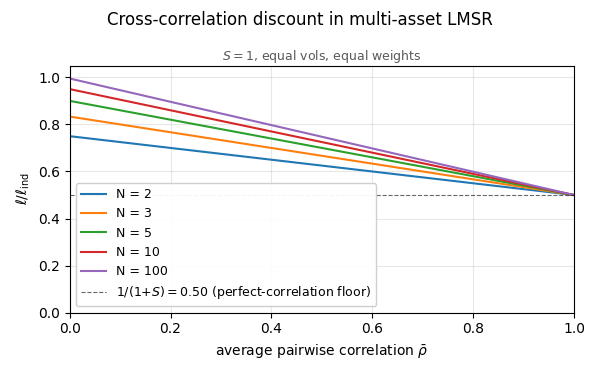
\includegraphics[width=0.85\textwidth]{lvr-multiasset-lmsr-fig.png}
\caption{Ratio of multi-asset LMSR LVR to the independent-pair benchmark as a function of average pairwise correlation, for a balanced pool $S=1$ and $N \in \{2, 3, 5, 10, 100\}$. All curves collapse to the floor $1/(1+S) = 0.5$ at perfect correlation.}
\label{fig:correlation}
\end{figure}

\subsection{Pool without num\'eraire}\label{sec:nocash}

If the LMSR pool holds only risky assets, with no num\'eraire, no asset has a fixed external price. Arbitrage equilibrates only the \emph{relative} prices: $p_i/p_j = P_i/P_j$ for every $i, j$, giving $p_i(q^\star) = P_i/T$ with $T \equiv \sum_{i=1}^N P_i$. Repeating \S\S\ref{sec:value}--\ref{sec:lvr} with the cash leg removed yields
\[
V_{\nc}(P) \;=\; b\,T \log T \;-\; b\sum_{i=1}^N P_i \log P_i \pmod{\text{linear in }P}, \qquad H_{ij}^{\nc}(P) \;=\; \frac{b}{T} \;-\; \frac{b}{P_i}\,\delta_{ij},
\]
\begin{equation*}
\ell_{\nc}(P) \;=\; \frac{b}{2}\Bigl[\sum_i \sigma_i^2 P_i \;-\; \frac{P\transp\Sigma P}{T}\Bigr] \;=\; \frac{b}{2}\sum_{i=1}^N P_i\,\sigma_{i,\rel,\nc}^2, \tag{10}
\end{equation*}
where in the last equality $\bar r_{\nc} = (P/T)\transp r$ is the value-weighted basket return \emph{within the risky leg} and $\sigma_{i,\rel,\nc}^2 = \Var(r_i - \bar r_{\nc})$. (The algebraic step is identity~$(\star)$ applied with $T$ in place of $S$.) That is, a no-num\'eraire LMSR's LVR rate consists \emph{only} of the relative-mode contribution: with no cash to arbitrage against, the common-mode channel is structurally absent.

\begin{corollary}\label{cor:zero}
Under perfectly correlated equal-volatility log-returns $d\log P_i = dX_t$ for every $i$ (a common Brownian-motion driver), $r_i \equiv \bar r_{\nc}$ a.s.\ for every $i$, so $\sigma_{i,\rel,\nc}^2 = 0$ and
\begin{equation*}
\boxed{\;\; \ell_{\rho=1}^{\,\nc} \;=\; 0. \;\;} \tag{11}
\end{equation*}
\end{corollary}

A no-num\'eraire LMSR of perfectly correlated assets suffers zero LVR. The argument is direct: collinear log-returns imply all $P_i$ scale by the same factor $\exp(X_t - X_0)$, so the ratios $P_i/P_j$ are constant, and the pool's marginal prices $p_i = P_i/T$ --- which depend only on those ratios --- never move. No arbitrage opportunity is ever generated. The cross-correlation discount has consumed the entire LVR.

This is the strongest expression of the LMSR cross-correlation effect, and Proposition~\ref{prop:sep} implies it cannot be replicated by any system of disjoint bilateral CFMM pools: with diagonal Hessian, $\ell_{\sep} > 0$ whenever any $\sigma_i^2 > 0$.

\section{Conclusion}\label{sec:conclusion}

We have derived in closed form the instantaneous LVR rate of the multi-asset Hanson LMSR with $N$ risky assets and one num\'eraire under idealized continuous arbitrage, eq.~$(\dagger)$. The rate decomposes as the sum of $N$ independent two-asset LMSR LVR rates minus the \emph{cross-correlation discount}
\[
\Delta(P) \;=\; \frac{b}{2(1+S)}\, P\transp\Sigma P,
\]
non-negative for any PSD return-covariance matrix and growing with the value-weighted basket-return variance.

Equivalently, by Theorem~\ref{thm:cm}, the rate splits orthogonally into a relative-mode contribution and a single common-mode contribution,
\[
\ell(P) \;=\; \frac{b}{2}\sum_i P_i\,\Var(r_i - \bar r) \;+\; \frac{b\,S}{2(1+S)}\,\Var(\bar r),
\]
making explicit that LMSR's shared simplex filters out the basket-direction common mode: the value-weighted-basket contribution to LVR is captured exactly once, as if the basket were a single synthetic asset, regardless of how many constituents the pool holds.

Three consequences are immediate. First, for perfectly correlated equal-volatility risky assets, $\Var(r_i - \bar r) = 0$ for every $i$, so the relative-mode contribution vanishes and the multi-asset rate collapses to the two-asset value (eq.~8). Second, without a num\'eraire the common-mode channel is structurally absent and only the relative-mode term survives (eq.~10); under perfect correlation, that term too vanishes, giving exactly zero LVR (eq.~11). Third, by Proposition~\ref{prop:sep}, no system of separable bilateral CFMMs --- whatever the choice of bilateral curvatures --- can exhibit a discount of this form, because separable value functions have diagonal Hessian and LVR depends only on the diagonal entries of $\Sigma$.

The effect is geometric: it descends from the off-diagonal simplex-coupling term in $\nabla^2 V$ induced by the constraint $\sum p_i = 1$. The practical implication for AMM design is that multi-asset LMSR pools assembled from highly correlated baskets --- liquid-staking derivatives of a common underlying, stablecoins of a single currency, share-class tokens of a single fund --- incur materially lower LVR (in the idealized continuous-arbitrage sense quantified above) per unit of liquidity depth than would the same assets split across bilateral pools. We emphasize that this is a statement about \emph{geometric adverse-selection exposure}, not about realized LP profitability: latency, gas, fees, and discrete arbitrage cadence all enter on top of the discount derived here and are not analyzed in this note.

Natural extensions --- fee-mediated LVR realization, discrete arbitrage cadence, the liquidity-sensitive LS-LMSR variant of Othman et al.\ (2010), and alternative multi-asset CFMM constructions with low-rank off-diagonal Hessians --- may preserve related geometric structure, but we do not establish here that the precise form of the discount derived above survives in any of those settings. Such extensions, and a characterization of the full class of multi-asset CFMMs admitting an analogous covariance-canceling discount, are natural follow-up questions outside the scope of this note.

\section*{References}

\begin{itemize}\setlength{\itemsep}{0pt}
\item Abernethy, J., Chen, Y., \& Vaughan, J.~W. (2013). Efficient market making via convex optimization, and a connection to online learning. \emph{ACM Transactions on Economics and Computation}, 1(2), 12.
\item Frongillo, R., \& Reid, M.~D. (2015). Convergence analysis of prediction markets via randomized subspace descent. In \emph{Advances in Neural Information Processing Systems} (NeurIPS).
\item Hanson, R. (2003). Combinatorial information market design. \emph{Information Systems Frontiers}, 5(1), 107--119.
\item Hanson, R. (2007). Logarithmic market scoring rules for modular combinatorial information aggregation. \emph{Journal of Prediction Markets}, 1(1), 3--15.
\item Milionis, J., Moallemi, C.~C., Roughgarden, T., \& Zhang, A.~L. (2024). Automated market making and loss-versus-rebalancing. arXiv:2208.06046.
\item Othman, A., Pennock, D.~M., Reeves, D.~M., \& Sandholm, T. (2010). A practical liquidity-sensitive automated market maker. In \emph{Proceedings of the 11th ACM Conference on Electronic Commerce (EC '10)}, 377--386.
\end{itemize}

\end{document}
